%   DOCUMENT CLASS  %%%%%%%%%%%%%%%%%%%%%%%%%%%%%%%%%%%%%%%%%%%%%%%%%%%%%%%%%%%
%
%   Use the `sfuthesis` class to format your thesis. If your program does not
%   require a thesis defence, use the class option `undefended` like so:
%
%     \documentclass[undefended]{sfuthesis}
%
%   To generate a signature page for your defence, use the `sfuapproval` class
%   instead, by replacing the below line with
%
%     \documentclass{sfuapproval}
%
%   For more information about thesis formatting requirements, go to
%
%     http://www.lib.sfu.ca/help/publish/thesis
%
%   or ask a thesis advisor at the SFU Research Commons.
%

\documentclass{sfuthesis}



%   DOCUMENT METADATA  %%%%%%%%%%%%%%%%%%%%%%%%%%%%%%%%%%%%%%%%%%%%%%%%%%%%%%%%
%
%   Fill in the following information for the title page and approval page.
%

\title{An example of a thesis or dissertation on the subject of your degree}
\thesistype{Thesis}
\author{Stuart Arthur Dent}
\previousdegrees{%
	M.Sc., Wossamotta University, 1963\\
	B.Sc., Unseen University, 1836}
\degree{Doctor of Philosophy}
\discipline{Mathematics}
\department{Department of Inadvisably Applied Mathematics}
\faculty{Faculty of Mad Science}
\copyrightyear{2017}
\semester{Spring 2017}
\date{January 10, 2017}

\keywords{thesis template; Simon Fraser University; time travel paradoxes}

\committee{%
	\chair{Pamela Isely}{Professor}
	\member{Emmett Brown}{Senior Supervisor\\Professor}
	\member{Bonnibel Bubblegum}{Supervisor\\Associate Professor}
	\member{James Moriarty}{Supervisor\\Adjunct Professor}
	\member{Kaylee Frye}{Internal Examiner\\Assistant Professor\\School of Engineering Science}
	\member{Hubert J.\ Farnsworth}{External Examiner\\Professor\\Department of Quantum Fields\\Mars University}
}



%   PACKAGES %%%%%%%%%%%%%%%%%%%%%%%%%%%%%%%%%%%%%%%%%%%%%%%%%%%%%%%%%%%%%%%%%%
%
%   Add any packages you need for your thesis here.
%   You don't need to call the following packages, which are already called in
%   the sfuthesis class file:
%
%   - appendix
%   - etoolbox
%   - fontenc
%   - geometry
%   - lmodern
%   - nowidow
%   - setspace
%   - tocloft
%
%   If you call one of the above packages (or one of their dependencies) with
%   options, you may get a "Option clash" LaTeX error. If you get this error,
%   you can fix it by removing your copy of \usepackage and passing the options
%   you need by adding
%
%       \PassOptionsToPackage{<options>}{<package>}
%
%   before \documentclass{sfuthesis}.
%
%   The following packages are a few suggestions you might find useful.
%
%   (1) amsmath and amssymb are essential if you have math in your thesis;
%       they provide useful commands like ``blackboard bold'' symbols and
%       environments for aligning equations.
%   (2) amsthm includes allows you to easily change the style and numbering of
%       theorems. It also provides an environment for proofs.
%   (3) graphicx allows you to add images with \includegraphics{filename}.
%   (4) hyperref turns your citations and cross-references into clickable
%       links, and adds metadata to the compiled PDF.
%   (5) pdfpages lets you import pages of external PDFs using the command
%       \includepdf{filename}. You will need to do this if your research
%       requires an Ethics Statement.
%

\usepackage{amsmath}                            % (1)
\usepackage{amssymb}                            % (1)
\usepackage{amsthm}                             % (2)
\usepackage{graphicx}                           % (3)
\usepackage{multirow}
\usepackage[pdfborder={0 0 0}]{hyperref}        % (4)
% \usepackage{pdfpages}                         % (5)
% ...
% ...
% ...
% ... add your own packages here!




%   OTHER CUSTOMIZATIONS %%%%%%%%%%%%%%%%%%%%%%%%%%%%%%%%%%%%%%%%%%%%%%%%%%%%%%
%
%   Add any packages you need for your thesis here. We've started you off with
%   a few suggestions.
%
%   (1) Use a single word space between sentences. If you disable this, you
%       will have to manually control spacing around abbreviations.
%   (2) Correct the capitalization of "Chapter" and "Section" if you use the
%       \autoref macro from the `hyperref` package.
%   (3) The LaTeX thesis template defaults to one-and-a-half line spacing. If
%       your supervisor prefers double-spacing, you can redefine the
%       \defaultspacing command.
%

\frenchspacing                                    % (1)
\renewcommand*{\chapterautorefname}{Chapter}      % (2)
\renewcommand*{\sectionautorefname}{Section}      % (2)
\renewcommand*{\subsectionautorefname}{Section}   % (2)
% \renewcommand{\defaultspacing}{\doublespacing}  % (3)
% ...
% ...
% ...
% ... add your own customizations here!




%   FRONTMATTER  %%%%%%%%%%%%%%%%%%%%%%%%%%%%%%%%%%%%%%%%%%%%%%%%%%%%%%%%%%%%%%
%
%   Title page, committee page, copyright declaration, abstract,
%   dedication, acknowledgements, table of contents, etc.
%
%   If your research requires an Ethics Statement, download one from the
%   SFU library website and uncomment the appropriate lines below.
%

\begin{document}

\frontmatter
\maketitle{}
\makecommittee{}

\begin{abstract}
	This is a blank document from which you can start writing your thesis.
\end{abstract}


\begin{dedication}
	This is an optional page.
\end{dedication}


\begin{acknowledgements}
	This is an optional page.
\end{acknowledgements}

\addtoToC{Table of Contents}%
\tableofcontents%
\clearpage

\addtoToC{List of Tables}%
\listoftables%
\clearpage

\addtoToC{List of Figures}%
\listoffigures%
\clearpage





%   MAIN MATTER  %%%%%%%%%%%%%%%%%%%%%%%%%%%%%%%%%%%%%%%%%%%%%%%%%%%%%%%%%%%%%%
%
%   Start writing your thesis --- or start \include ing chapters --- here.
%

\mainmatter%

%\chapter{Introduction}

%By default, only works cited in the text will be added to the bibliography~\cite{latexcompanion}.

\chapter{Results}

\section{Comparing Action Values between models}

We compare action values computed by the different models of the home serve action for all possible outcomes. Note that there is no inherent order in the outcome symbols, the values for the different outcomes are entirely learned by the models.

\begin{table}[]
	\centering
	\begin{tabular}{c|ccccc}
		\multirow{2}{*}{\textbf{Serve Outcome}} & \multicolumn{5}{c}{\textbf{Home Win Probability}}                                                            \\
		& \textbf{Dec. Tree} & \textbf{Rand. Forest} & \textbf{Neural Net.} & \textbf{Mimic Tree} & \textbf{From Data} \\ \hline
		\textbf{=}                              & 0                  & 0                     & 0.1                  & 0.1                 & 0                  \\
		\textbf{-}                              & 35.4               & 35.4                  & 35.5                 & 35.5                & 35.4               \\
		\textbf{!}                              & 55.2               & 50.6                  & 44.9                 & 44.9                & 44.7               \\
		\textbf{+}                              & 55.2               & 62.3                  & 61.2                 & 61.2                & 61.9               \\
		\textbf{\#}                             & 100                & 100                   & 99.9                 & 99.9                & 100               
	\end{tabular}
	\caption{Mean home win probabilities (in percent) for the home serve action type broken down by outcome. Comparison between different models and win probability obtained from dataset.}
	\label{tab:serve-values}
\end{table}

\section{Verifying Bellman Equation Agreement}

The action-value function $Q_\pi$ for a given policy $\pi$ over a Markov decision process satisfies a recursive relationship in terms of the current state-action pair $(s,a)$ and possible future state-action pairs $(S_{t+1},A_{t+1})$: 
\begin{align}
Q_\pi(s,a) &= \mathbb{E} \left[  R_{t+1} + \gamma Q_{\pi}(S_{t+1}, A_{t+1}) \, | \, S_t = s, A_t = a \right]\\
&=  R_{t+1} + \sum_{s' \in S, a' \in A} \gamma P(S_{t+1} = s', A_{t+1} = a' | S_t = s, A_t = a) Q_\pi(s',a').
\end{align}
This property is known as the Bellman equation \cite{sutton2018reinforcement} and it gives us the opportunity to verify the quality of our action-value estimates in an aspect that is different from what we did so far. If our approximation is indeed an action-value function, we expect it to (at least approximately) agree with the Bellman equation in addition to minimizing the loss function against the training data.\\\\
In our context we use a discount factor of $\gamma = 1$ and rewards only occur at episode-ending states. If $s$ is not a terminal state, $R_{t+1} = 0$ and the Bellman equation becomes
\begin{equation}
Q(s,a) = \sum_{s',a'} P(S_{t+1} = s', A_{t+1} = a' | S_t = s, A_t = a) Q(s',a').
\label{eq:markov_diff}
\end{equation}
Assuming we've computed an action-value function estimate for all the states in our dataset, we can proceed to verify this equality using the data, since the transition probability $P$ can be estimated by counting occurrences of states in the dataset (denoted by $c$) as
$$P(S_{t+1} = s', A_{t+1} = a' | S_t = s, A_t = a) = \frac{c(S_{t+1} = s', A_{t+1} = a', S_t = s, A_t = a)}{c(s,a)}.$$
Furthermore, since the state space is large, we wish to avoid examining a single state due to potential data sparsity effects. We will instead be interested in a set of state-action pairs $X$, summing all the corresponding state-action values as they appear in the dataset, namely the quantity:
$$\sum_{s,a\in X} c(s,a)Q(s,a).$$
Using \eqref{eq:markov_diff}, we obtain the right hand side:
\begin{equation}
\sum_{s,a\in X} c(s,a)Q(s,a) = \sum_{s,a\in X} c(s,a)\sum_{s',a'\in S\times A} \frac{c(s',a',s,a)}{c(s,a)} Q(s',a'),
\end{equation}
which simplifies to
\begin{equation}
\sum_{s,a\in X} c(s,a)Q(s,a) = \sum_{s,a\in X} \sum_{s',a'\in S\times A} c(s',a',s,a) Q(s',a').
\label{eq:markov_num}
\end{equation}
This final form is the one we use to compute the Bellman equation agreement, since both the left and right hand sides can be computed in a simple loop over the dataset sequences. We are interested in how much our action-value estimates violate \eqref{eq:markov_num}, i.e. the quantity
\begin{equation}
e_X = |\sum_{s,a\in X} c(s,a)Q(s,a) - \sum_{s,a\in X} \sum_{s',a'\in S\times A} c(s',a',s,a) Q(s',a') |.
\label{eq:markov_num2}
\end{equation}
We choose the state-action subset $X$ to include actions of a single type with only non-terminal outcomes (for example, we include all serve actions that do not result in an immediate error or point won). We compute the quantity $e_X$ for various action types and compare results across different action-value function approximations.\\\\
Looking at the $e_X$ values shown in Table \ref{tab:bellman-agreement}, the neural network exhibits overall highest agreement with the Bellman equation and the single decision tree is the worst of our models in this respect. Since the neural network is trained using reinforcement learning principles, in particular because the loss function incorporates the temporal difference target 
$$Q(s,a) \leftarrow Q(s,a) + \alpha (r + \gamma Q(s', a') - Q(s,a)),$$
where the state-action pair $(s,a)$ is followed by $(s',a')$ in the data, it is not surprising that temporal consistency is best maintained using this model. Decision tree and random forest models are trained under the assumption of independent data and do not incorporate any information about the sequential nature of the volleyball data. Their $e_X$ values are accordingly much larger and in the case of random forest could outweigh its lower mean squared error compared to the neural network. The mimic tree's $e_X$ seems to be close to the neural network's in most cases, but significantly higher for attack and block actions, which puts it somewhere between the neural network and the random forest overall.

\begin{table}[]
	\centering
	\begin{tabular}{c|cccccc}
		\textbf{Model}    & \textbf{Serve} & \textbf{Receive} & \textbf{Attack} & \textbf{Set} & \textbf{Block} & \textbf{Dig} \\ \hline
		Decision Tree     & 0.0158                  & 0.0151                    & 0.0376                   & 0.0074                & 0.0641                  & 0.0662                \\
		Random Forest     & 0.0172                  & 0.0183                    & 0.0075                   & 0.0066                & 0.0025                  & 0.0148                \\
		RL Neural Network & 0.0001                  & 0.0005                    & 0.0003                   & 0.0019                & 0.0008                  & 0.0002                \\
		Mimic Tree        & 0.0001                  & 0.0001                    & 0.0076                   & 0.0018                & 0.0125                  & 0.0009               
	\end{tabular}
	\caption{Table of Bellman equation agreement error $e_X$ for various sets of non-terminal states $X$. For each volleyball action type (columns), the set $X$ includes actions performed by the home team with a non-terminal outcome.}
	\label{tab:bellman-agreement}
\end{table}

\section{Action Impact}

One of the motivations of computing the action-value function for sports data is the ability to numerically rank teams and players according to their action values. To achieve this, we need to consider that the context of an action performed by a player influences the quality of their actions. Namely, scoring a point from a favorable situation (eg. a successful attack following a perfect pass) should be treated differently than scoring in a situation that is deemed difficult. This leads us to the notion of action impact.\\\\
As discussed in \cite{routley2015markov}, there are several options of how we could choose to value actions. We will adopt the difference of consecutive action values as a measure of impact. Namely, for a transition from state $s_{t-1}$ to $s_t$, with actions $a_{t-1}$ and $a_t$ we define the impact of $(s_t, a_t)$ as:
\begin{equation}
\text{impact}(s_t,a_t) = Q(s_t,a_t) - Q(s_{t-1},a_{t-1}).
\label{eq:action_impact}
\end{equation}
This allows us to capture to some degree how the flow of the game changed when action $a_t$ was performed. This version of valuing player actions was successfully used in the hockey context in \cite{liu2018deep} for player evaluations.\\\\
Note that since action impact relates to the values of both current and previous states, we need to find a treatment for the first action of any episode (in volleyball this is always a serve action), where $s_{t-1}$ and $a_{t-1}$ are not defined. The most obvious solution is to use an initial state-action value of 0, but since the serving team is generally at a disadvantage in terms of scoring probability, this approach gives serve actions a negative value on average and renders serve values disproportionate when compared to other action types. We therefore proceed as follows. Define $Q_{SH}$ to be the mean value of all home serve actions and $Q_{SA}$ to be the mean value of all away serve actions. We then use these values to compute action impacts as:
\begin{equation}
\text{impact}(s_t,a_t) =
	\begin{cases} 
	Q(s_t,a_t) - Q_{SH} & \text{if } a_t \text{ is home serve,} \\
	Q(s_t,a_t) - Q_{SA} & \text{if } a_t \text{ is away serve,} \\
	Q(s_t,a_t) - Q(s_{t-1},a_{t-1}) & \text{otherwise.} 
	\end{cases}
	\label{eq:action_impact2}
\end{equation}
The intuition behind this approach is to have the serve impact measure the difference between the current serve and the average serve. We also know the home team tends to have a slight advantage, which is the reason for separate averaging of home and away serves. The two means, $Q_H$ and $Q_A$ do in fact differ in absolute value by about 0.06 in favour of the home team.\\\\
Firstly, we consider team collective action impact and investigate how well it aligns with team performance in the Canada West volleyball competition in the last three seasons. To this end, we compute the mean impact of all actions performed by players of a particular team using equation \eqref{eq:action_impact2}. These values are collected in Table \ref{tab:team-impact} for all teams participating in the Canada West men's volleyball competition (with the exception of Regina, who ceased participation after the 2017/2018 season and is not well represented in the dataset). We compare action impact values to mean ranking of the teams following regular season across the 2017/2018, 2018/2019 and 2019/2020 seasons, also included in Table \ref{tab:team-impact}. Teams in the table are sorted by mean action impact. Good alignment against team ranking can be seen from inspection of the table, but a plot is also included in Figure \ref{fig:team-impact} for a more visual representation. With the exception of three teams, an increase in mean action impact corresponds to higher ranking, which is desirable behaviour for our model, as higher action values lead to more wins. We also compute the Pearson correlation coefficient between mean action impacts and mean rankings and obtain a value of -0.854, confirming a high correlation and a near linear relationship.\\
\begin{table}[h]
	\centering
	\begin{tabular}{cccccc}
		\textbf{Team}   & \textbf{Mean Action Impact} & \textbf{R20} & \textbf{R19} & \textbf{R18} & \textbf{Mean Ranking} \\ \hline
		Trinity Western & 0.0220                      & 1            & 2            & 1            & 1.33                  \\
		Alberta         & 0.0175                      & 2            & 3            & 3            & 2.67                  \\
		UBC             & 0.0124                      & 3            & 7            & 2            & 4.00                  \\
		Brandon         & 0.0077                      & 4            & 1            & 4            & 3.00                  \\
		Calgary         & 0.0073                      & 5            & 8            & 6            & 6.33                  \\
		Winnipeg        & 0.0053                      & 6            & 10           & 5            & 7.00                  \\
		Mount Royal     & -0.0053                     & 8            & 4            & 10           & 7.33                  \\
		Manitoba        & -0.0067                     & 10           & 9            & 7            & 8.67                  \\
		MacEwan         & -0.0128                     & 12           & 11           & 12           & 11.67                 \\
		Thompson Rivers & -0.0144                     & 9            & 6            & 8            & 7.67                  \\
		Saskatchewan    & -0.0210                     & 7            & 5            & 9            & 7.00                  \\
		UBCO            & -0.0235                     & 11           & 12           & 11           & 11.33                
	\end{tabular}
	\caption{Canada West teams sorted by mean action impact. Columns R20, R19, R18 are team rankings after regular season in 2020, 2019 and 2018, respectively and Mean Ranking is the mean of those three columns.}
	\label{tab:team-impact}
\end{table}\\
We note here again that the dataset contains all UBC games, but not all games among other Canada West teams, meaning that the amount of data for those teams is significantly lower than for UBC. The bias introduced by this could explain the outliers in Figure \ref{fig:team-impact}.\\\\
We can compute mean action impacts for individual players in the same fashion as we did for teams above, which enables us to track and rank player performance. Table \ref{tab:player-impact} shows the top 10 players ranked by mean action impact in Canada West. The caveat, compared to team ranking, is that there are fewer obvious ways to check the validity of these values. In professional leagues such as the NHL, player salary has been used for this purpose, e.g. in \cite{schulte2017apples}, but there is no such information for university athletes. Regardless, we still attempt some discussion. Notably, most of the players listed come from the top ranked teams - the best 4 teams in Canada West (by mean ranking in the last 3 seasons) are represented 8 out of 10 times, which can be taken as a good sign.\\\\
On a more individual level, player awards and recognition can provide further validity to our ranking. Elliot Viles, who ranks first in Table \ref{tab:player-impact}, was named a conference all-star in his rookie season and both Canada West as well as U SPORTS National player of the year in the 2018/2019 season. He also represented his home country Australia in the prestigious FIVB World League competition. Eric Loeppky, who follows closely in the mean impact ranking, also received the title of U SPORTS player of the year in 2020 as well as multiple other awards and has played on the Canadian senior national team, which is rare for players still in their university years. Jackson Kennedy and Daniel Thiessen have furthermore been selected as Canada West all-star team members alongside Loeppky and Viles. Prominent players like that featuring as leaders in impact ranking is further validation of our action impact model.
\begin{table}[]
	\centering
	\begin{tabular}{ccc}
		\textbf{Player Name} & \textbf{Team}   & \textbf{Mean Action Impact} \\ \hline
		Elliot Viles         & Brandon         & 0.0838                      \\
		Eric Loeppky         & Trinity Western & 0.0796                      \\
		Jackson Kennedy      & Alberta         & 0.0580                      \\
		George Hobern        & Alberta         & 0.0566                      \\
		Hamish Hazelden      & Calgary         & 0.0539                      \\
		Joel Regher          & UBC             & 0.0509                      \\
		Daniel Thiessen      & Winnipeg        & 0.0504                      \\
		Gerard Murray        & UBC             & 0.0471                      \\
		Jordan Canham        & Alberta         & 0.0459                      \\
		Arran Chambers       & Alberta         & 0.0451                     
	\end{tabular}
	\caption{Top 10 individual players in Canada West by mean action impact as given in equation \eqref{eq:action_impact2}.}
	\label{tab:player-impact}
\end{table}



\begin{figure}
	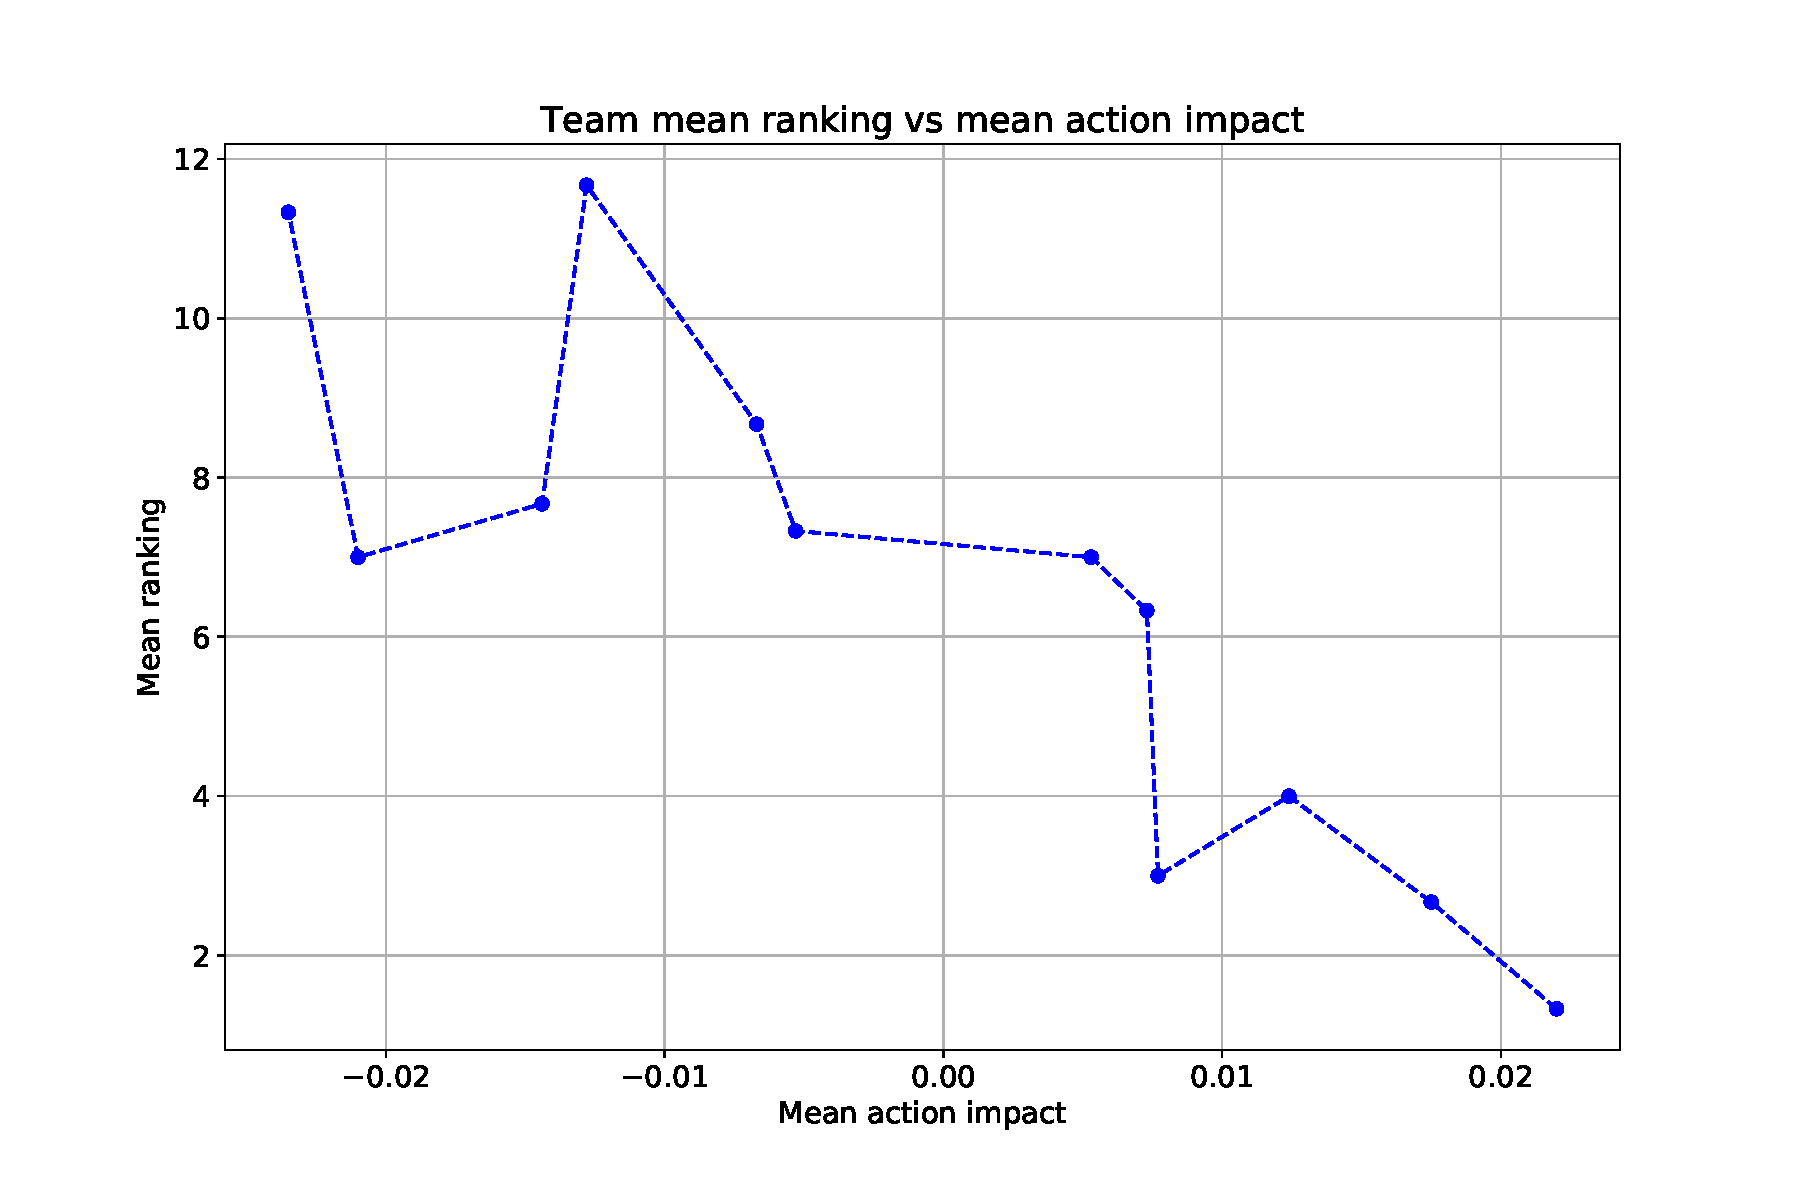
\includegraphics[scale=0.55]{img/team_ranking.pdf}
	\caption{Team mean ranking plotted against mean action impact for Canada West participating teams, see Table \ref{tab:team-impact} for values shown in this graph.}
	\label{fig:team-impact}
\end{figure}

%   BACK MATTER  %%%%%%%%%%%%%%%%%%%%%%%%%%%%%%%%%%%%%%%%%%%%%%%%%%%%%%%%%%%%%%
%
%   References and appendices. Appendices come after the bibliography and
%   should be in the order that they are referred to in the text.
%
%   If you include figures, etc. in an appendix, be sure to use
%
%       \caption[]{...}
%
%   to make sure they are not listed in the List of Figures.
%

\backmatter%
	\addtoToC{Bibliography}
	\bibliographystyle{plain}
	\bibliography{msc_report}

\begin{appendices} % optional
	\chapter{Code}
\end{appendices}
\end{document}
